As gravitational waves from the merger of two black holes were detected in 2015, for the first time by the Advanced Laser Interferometry Gravitational-Wave Observatory (aLIGO) which spiked the interest in computational frameworks for computational general relativity, which enables to perform simulation on binary black hole merger problem. In this project, we would like to focus on developing an efficient, scalable visualization pipeline for our own research code Dendro(please note that current work is not published yet, but an extension of \cite{Fernando:2017:MAA:3078597.3078610}) which enables to solve BSSN\cite{2012PhRvD..85h4004B} formulation of Einstien equations in an efficient scalable manner, using octree based adaptive mesh refinement and with adaptive time stepping. 

BSSN formulation consists of $24$ non-linear hyperbolic PDE decomposition of Einstien equations which enables stable numerical time stepping. Hence each data files consists of $24$ evolution variables and $6$ constraint equations which are being used to test the physical validity of the solution. 

\begin{figure}[H]
	\centering
	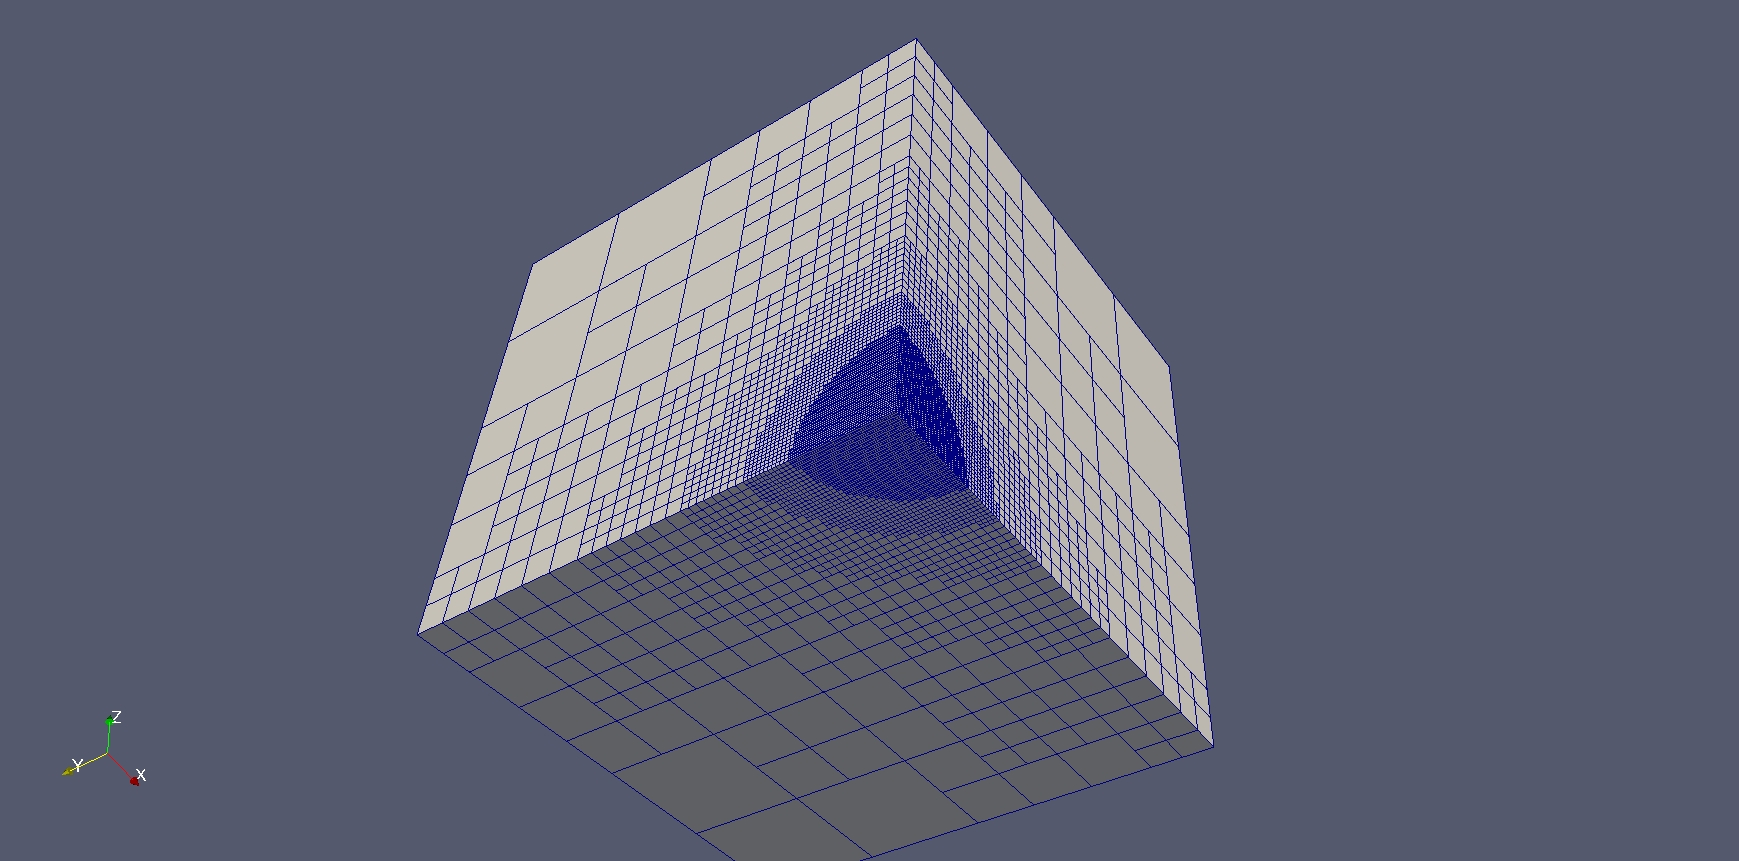
\includegraphics[width=0.45\textwidth]{figs/aoctree.jpg}  \hfill
	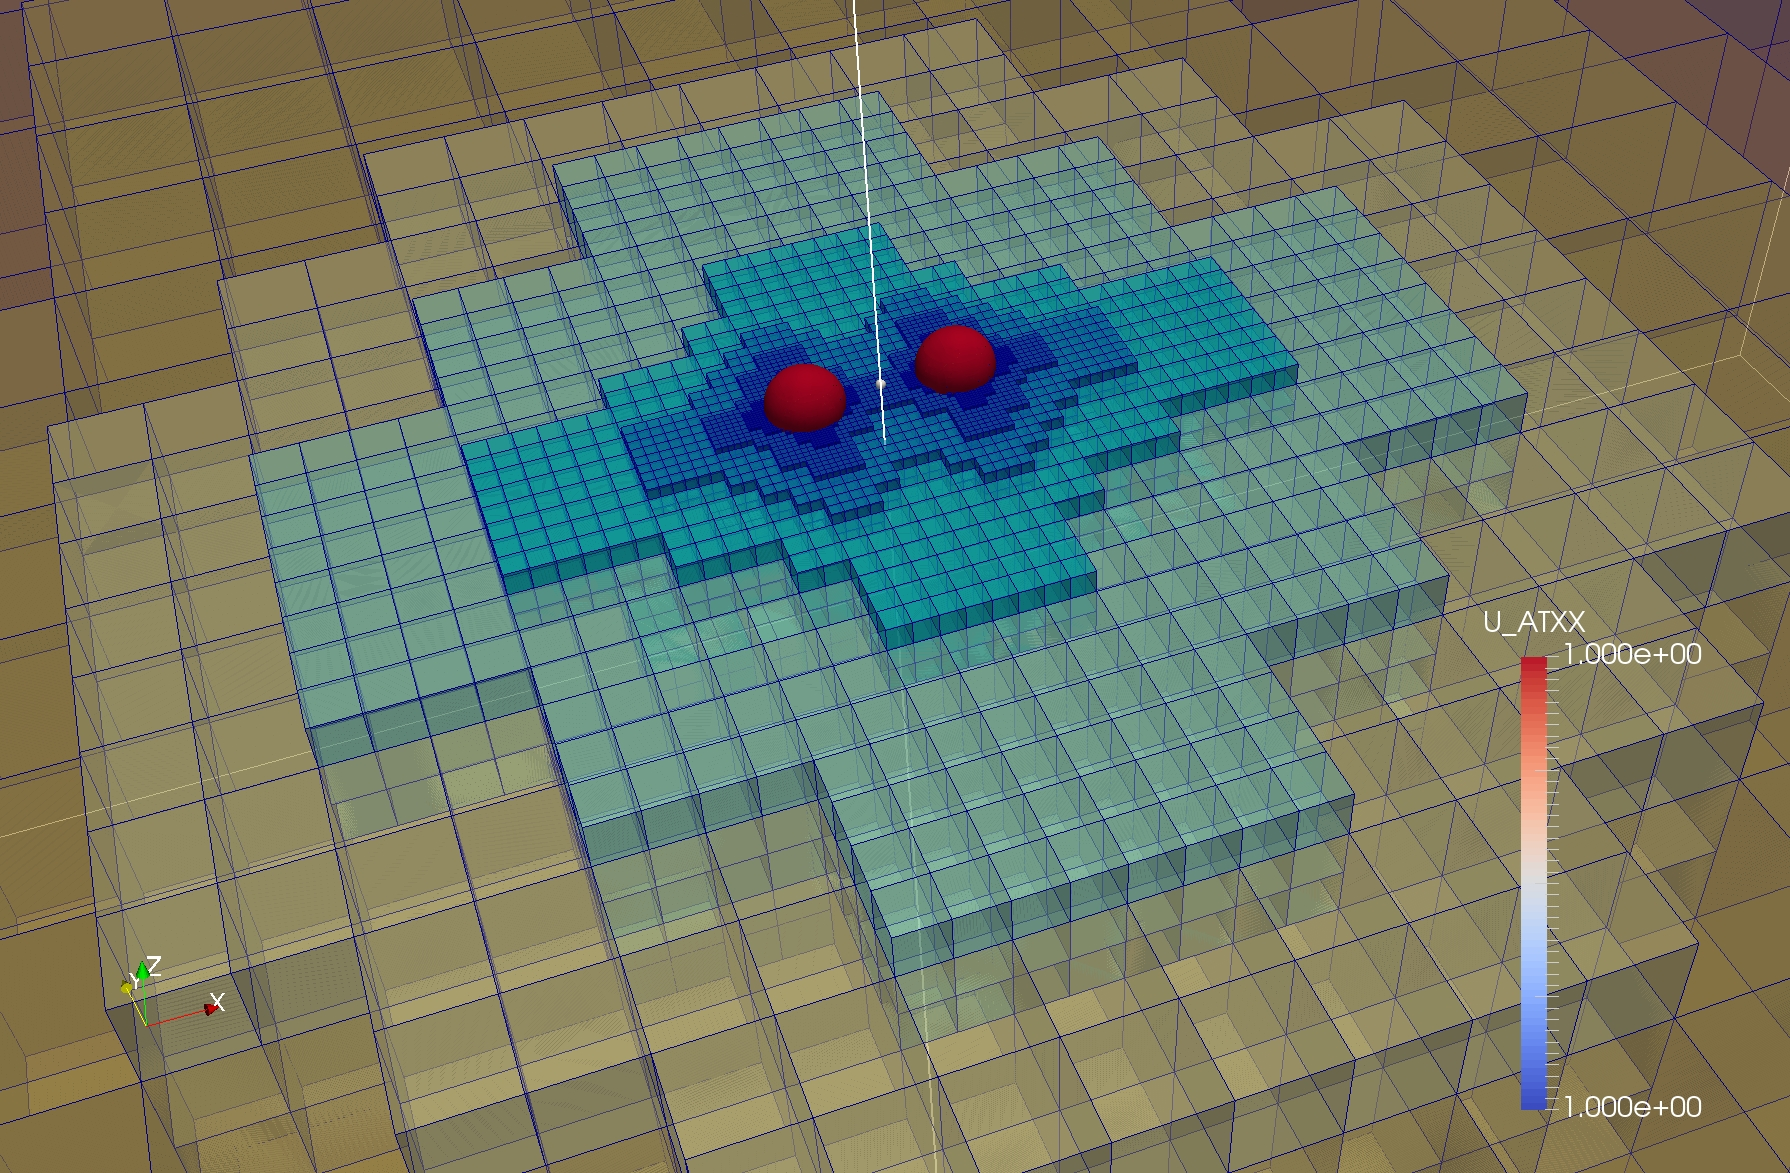
\includegraphics[width=0.45\textwidth]{figs/bh_image.jpg}
	\caption{\label{fig:octree} The leftmost figure shows an example of adaptive $2:1$ balanced octree and the rightmost image shows underlying adaptive grid for equal mass binary black hole problem.  }
\end{figure}